%% Template for ENG 401 reports
%% by Robin Turner
%% Adapted from the IEEE peer review template

\documentclass[journal,12pt,onecolumn,a4paper]{IEEEtran}
\usepackage{cite} % Tidies up citation numbers.
\usepackage{url} % Provides better formatting of URLs.
\usepackage[utf8]{inputenc} % Allows Turkish characters.
\usepackage{booktabs} % Allows the use of \toprule, \midrule and \bottomrule in tables for horizontal lines
\usepackage{graphicx}
\usepackage{amsmath}
\usepackage{float}
\usepackage{multicol}
\usepackage{listings}
\usepackage[justification=centering]{caption}
\usepackage[numbered,framed]{matlab-prettifier}
\usepackage[export]{adjustbox}

\graphicspath{ {./assets/pics} }

\hyphenation{op-tical net-works semi-conduc-tor} % Corrects some bad hyphenation 
\lstset{
  basicstyle=\ttfamily,
  columns=fullflexible,
  breaklines=true,
  postbreak=\mbox{\textcolor{red}{$\hookrightarrow$}\space},
}


\begin{document}
\begin{titlepage}
	% paper title
	% can use linebreaks \\ within to get better formatting as desired
	\title{Interpolasi Numerik: Path Calculator}


	% author names and affiliations

	\author{Adrian Ardizza\\
		Alya Azhar Agharid\\
		Muhammad Athallah\\
		Stefanus Ndaru Wedhatama
	}

	% make the title area
	\maketitle
	\begin{abstract}
		The abstract does not only mention the paper but is the original paper shrunken to approximately 200 words. It states the purpose, reports the information obtained, and gives conclusions, and recommendations. In short, it summarizes the main points of the study adequately and accurately. It provides information from every major section in the body of the report in a dense and compact way. Past tense and active voice is appropriate when describing what was done. If there is any, it includes key statistical detail.

		Depending on the format you use, the abstract may come on the title page or at the beginning of the main report.

	\end{abstract}
	\tableofcontents
	\listoffigures
	\listoftables
\end{titlepage}

\IEEEpeerreviewmaketitle

\section{Pendahuluan}
Interpolasi merupakan teknik yang digunakan untuk membangun suatu fungsi yang melewati sebuah himpunan titik-titik diskret yang diketahui. Fungsi interpolasi memiliki aplikasi yang luas pada Ilmu Komputer karena dapat digunakan untuk menggambarkan berbagai kurva kompleks dengan \emph{computational cost} yang relatif murah apabila dibandingkan dengan metode brute-force (mencari seluruh titik yang memenuhi suatu kurva secara \emph{exhaustive}). Interpolasi beberapa titik diskret dapat dicapai dengan berbagai metode interpolasi seperti interpolasi konstan, interpolasi linear, interpolasi polinomial, dan interpolasi \emph{spline} yang menjadi topik dari paper ini.

Secara matematis, sebuah fungsi interpolasi dapat dinyatakan sebagai suatu fungsi \(P(x)\) dimana \(x\) adalah sebuah titik yang ingin di-interpolasi. Hasil dari fungsi tersebut adalah sebuah value yang merupakan aproksimasi dari nilai fungsi \(f(x)\) yang melewati seluruh titik-titik diskret yang nilainya sudah diketahui.

Pada paper ini, kami ingin mengeksplorasi pemanfaatan sebuah fungsi \emph{cubic spline} - atau lebih tepatnya fungsi \emph{cubic spline} dengan kondisi \emph{natural} - untuk melakukan \emph{smoothing} pada perubahan posisi suatu titik di interval waktu \([0, n]\). Cubic spline dapat didefinisikan sebagai suatu \emph{piecewise polynomial function} yang menginterpolasi sebuah himpunan titik dengan menggunakan sebuah \emph{cubic polynomial} sebagai fungsi dasarnya pada setiap interval.

Untuk sebuah input yang berisi \(n\) titik, akan terdapat \(n-1\) \emph{cubic function} yang menginterpolasi titik-titik tersebut di setiap interval. Pembangunan spline ini sendiri akan dijelaskan secara lebih mendetil pada bagian selanjutnya. Fungsi \emph{natural cubic spline} ini kemudian akan digunakan sebagai basis untuk suatu fungsi parametrik \((x(t), y(t))\) yang mengambil suatu array berisi time-step dengan resolusi \(r\) dan menginterpolasi (x, y) untuk input tersebut.

Output yang diharapkan dari fungsi tersebut adalah sebuah kurva parametrik  menginterpolasi gerak titik seperti pada dua contoh berikut ini:

\begin{multicols}{2}
	\begin{figure}[H]
		\centering
		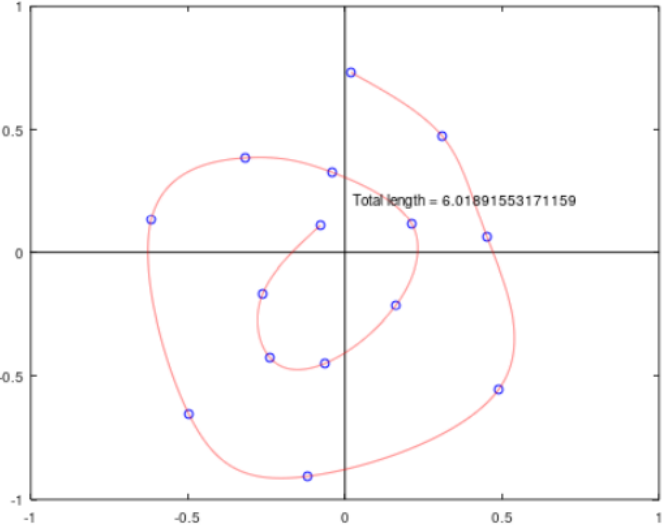
\includegraphics[max size={\textwidth/2}{\textheight}]{soal1-tc1}
		\caption{Contoh Graf Interpolasi \#1}
		\label{fig_sim2}
	\end{figure}
	\columnbreak
	\begin{figure}[H]
		\centering
		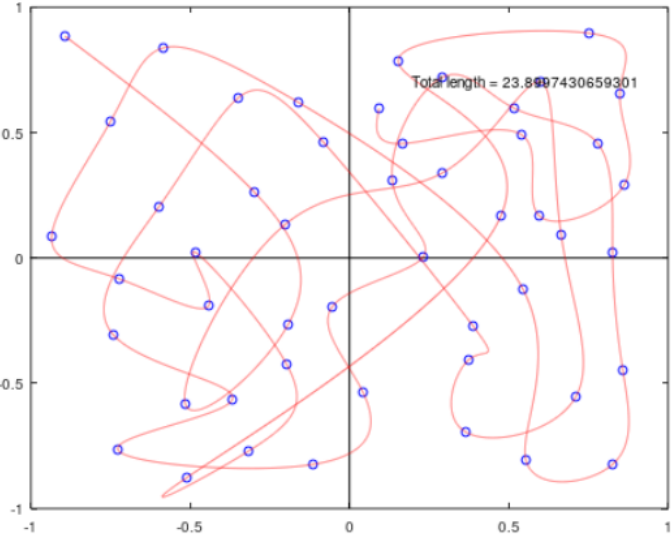
\includegraphics[max size={\textwidth/2}{\textheight}]{soal1-tc2}
		\caption{Contoh Graf Interpolasi \#2}
		\label{fig_sim2}
	\end{figure}
\end{multicols}

\pagebreak

\section{Membangun fungsi (x(t), y(t))}
Pada bagian ini, kami akan membangun fungsi parametrik \((x(t), y(t))\) yang dapat menghasilkan output yang diharapkan dari tugas kali ini.

\subsection{Definisi Cubic Spline}
Apabila diberikan \(n + 1\) titik data \(x_i, y_i\), dimana \(a = x_0\) dan \(b = x_n\), maka fungsi cubic spline \(S(x)\) adalah fungsi yang memenuhi syarat:
\begin{itemize}
	\item \(S(x) \in C^2[a, b]\)
	\item Pada setiap subinterval \([x_{i - 1}, x_i]\) dimana \(i = 1, ..., n\), \(S(x)\) adalah polinomial derajat 3.
	\item \(S(x_i) = y_i\) untuk semua \(i = 0, 1, ..., n\).
\end{itemize}

Sehingga kita dapat mendefinisikan fungsi \emph{cubic spline} \(S(x)\) sebagai:
\begin{equation}
	S(x) = \begin{cases}
		C_1(x) & x_0 \leq x \leq x_1  \\
		\dots                         \\
		C_i(x) & x_{i-1} < x \leq x_i \\
		\dots                         \\
		C_n(x) & x_{n-1} < x \leq x_n
	\end{cases}
\end{equation}
\begin{equation}
	\text{dimana }C_i = a_i + b_ix + c_ix^2 + d_ix^3
\end{equation}

Pada umumnya, sebuah \emph{cubic spline} harus memenuhi beberapa syarat:
\begin{itemize}
	\item Menginterpolasi titik-titik data: \(s_i(x_i) = y_i\)
	\item \(S(x)\) kontinu pada interval \([0, n]\): \(s_i{x_i+1} = y_{i + 1}\)
	\item Turunan pertama \(S(x)\) kontinu pada interval \([0, n]\): \(S_i'(x_{i + 1}) = s_{i + 1}'(x_{i + 1})\)
	\item Turunan kedua \(S(x)\) kontinu pada interval \([0, n]\): \(S_i''(x_{i + 1}) = S_{i + 1}''(x_{i + 1})\)
\end{itemize}

Selain itu, sebuah fungsi cubic spline juga harus memenuhi sebuah \emph{boundary condition} untuk membentuk suatu sistem persamaan yang dapat diselesaikan. Pada tugas kali ini, \emph{boundary condition} yang digunakan adalah kondisi \emph{natural} yang didefinisikan sebagai:
\begin{equation}
	S_0''(x_0) = 0
\end{equation}
\begin{equation}
	S_{n-1}''(x_n) = 0
\end{equation}

Dari syarat-syarat tersebut akan diperoleh suatu sistem persamaan linear yang dapat digunakan untuk mencari koefisien dari setiap \emph{piecewise cubic function} yang menginterpolasi interval \([a, b]\).

Setelah mendefinisikan syarat-syarat yang harus dipenuhi oleh \emph{cubic spline}, maka kita dapat mulai membangun definisi umum \emph{natural cubic spline} yang dapat diimplementasikan dengan menggunakan MATLAB. Terdapat dua pendekatan yang dapat dilakukan untuk membangun sistem ini, yakni secara \emph{top-down} ataupun secara \emph{bottom-up}.

Pendekatan \emph{top-down} dilakukan dengan mencari nilai-nilai koefisien \(a, b, c, d\) yang dapat memenuhi persamaan \(S_i(x) = a_i + b_ix + c_ix^2 + d_ix^3\). Pendekatan ini akan menghasilkan suatu sistem persamaan yang memiliki 4n \emph{unknowns} dan 4n \emph{equations}, dimana n adalah jumlah titik yang ingin di-interpolasi.

Sementara itu pendekatan \emph{bottom-up} dilakukan dengan pertama mendefinisikan sebuah fungsi \(S''(x)\) linear yang kemudian diintegrasikan untuk mendapatkan suatu fungsi \(S(x)\) kubik. Lalu kita dapat menggunakan syarat-syarat yang sudah didefinisikan pada bagian sebelumnya untuk mencari \emph{unknown terms} yang dihasilkan oleh proses integrasi dan mendefinisikan sistem persamaan yang mencari semua \emph{knot} pada \emph{spline} dan fungsi \emph{spline} pada setiap interval.

\subsection{Membangun Algoritma Natural Cubic Spline}
Kami akan menggunakan pendekatan \emph{bottom-up} untuk membangun algoritma Natural Cubic Spline yang akan digunakan pada fungsi \((x(t), y(t))\).

Asumsikan bahwa:
\begin{itemize}
	\item Kita memiliki suatu himpunan berisi \(n\) titik data \((x_i, y_i)\) dimana \(x_1 < x_2 < \dots < x_n\)
	\item \(f(x)\) adalah polinomial dengan derajat \(\leq 3\) pada setiap subinterval \([x_i, x_{i + 1}]\)
	\item \(f(x)\), \(f'(x)\), \(f''(x)\) adalah fungsi kontinu untuk interval \(a \leq x \leq b\) sehingga:
	      \begin{itemize}
		      \item \(f_{i-1,i}(x_i) = f_{i, i+1}(x_i)\)
		      \item \(f_{i-1,i}'(x_i) = f_{i, i+1}'(x_i)\)
		      \item \(f_{i-1,i}''(x_i) = f_{i, i+1}''(x_i)\ = k_i\)
	      \end{itemize}
	      Dimana \(k_i\) adalah nilai turunan kedua \(f(x)\) pada segmen ke-i
\end{itemize}

Dengan asumsi tersebut, kita dapat mulai membangun fungsi interpolant \(f_{i, i+1}(x)\) dengan asumsi fungsi tersebut adalah sebuah fungsi kubik. Karena fungsi tersebut merupakan suatu fungsi derajat tiga, maka turunan keduanya pada suatu \(x\) merupakan sebuah fungsi linear.

Ingat bahwa sebuah fungsi linear yang menginterpolasi 2 titik dapat dicari menggunakan basis Lagrange, sehingga kita dapat mendefinisikan \(S''(x)\) sebagai berikut:
\begin{equation*}
	f''_{i, i+1}(x) = k_i\frac{x-x_{i + 1}}{x_i - x_{i + 1}} + k_{i+1}\frac{x - x_i}{x_{i + 1} - x_i}
\end{equation*}

Selanjutnya, kita dapat melakukan integrasi pada fungsi tersebut untuk mendapatkan \(f_{i, i+1}'(x)\) dan \(f_{i, i+1}(x)\).
\begin{equation*}
	\begin{split}
		f_{i, i+1}'(x) & = \int f_{i, i+1}''(x) dx\\
		& = \int (k_i\frac{x-x_{i + 1}}{x_i - x_{i + 1}} + k_{i+1}\frac{x - x_i}{x_{i + 1} - x_i})dx\\
		& = \frac{k_i(x-x_{i+1})^2}{2(x_i-x_{i+1})} + \frac{k_{i+1}(x-x_{i})^2}{2(x_{i+1}-x_{i})} + C
	\end{split}
\end{equation*}
\begin{equation*}
	\begin{split}
		f_{i, i+1}(x) & = \int f_{i, i+1}'(x) dx\\
		& = \int (\frac{k_i(x-x_{i+1})^2}{2(x_i-x_{i+1})} + \frac{k_{i+1}(x-x_{i})^2}{2(x_{i+1}-x_{i})} + C)dx\\
		& = \frac{k_i(x-x_i)^3}{6(x_i - x_{i+1})} + \frac{k_{i+1}(x - x_i)^3}{6(x_{i+1} - x_i)} + Cx + D
	\end{split}
\end{equation*}

Setelah mendapatkan fungsi \(f(x)\) dan \(f'(x)\), kita harus selanjutnya mencari nilai dari suku C dan D agar dapat menggunakan fungsi tersebut sebagai interpolant.
\begin{equation*}
	\begin{split}
		C & = A - B\\
		D & = -Ax_{i+1} + Bx_i
	\end{split}
\end{equation*}

Sehingga kita akan mendapatkan,
\begin{equation*}
	\begin{split}
		f_{i, i+1}(x) & = \frac{k_i(x-x_i)^3}{6(x_i - x_{i+1})} + \frac{k_{i+1}(x - x_i)^3}{6(x_{i+1} - x_i)} + (A-B)x - Ax_{i+1} + Bx_i\\
		& = \frac{k_i(x-x_i)^3}{6(x_i - x_{i+1})} + \frac{k_{i+1}(x - x_i)^3}{6(x_{i+1} - x_i)} + A(x-x_{i+1}) - B(x-x_i)
	\end{split}
\end{equation*}

\section{Kesimpulan}
Kesimpulan disini.

% % Example of a table from http://www.latextemplates.com/template/professional-table

\begin{thebibliography}{1}
	% Here are a few examples of different citations 
	% Book
	\bibitem{kopka_1999} % Note the label in the curly brackets. Use the cite the source; e.g., \cite{kopka_latex}
	H.~Kopka and P.~W. Daly, \emph{A Guide to \LaTeX}, 3rd~ed.\hskip 1em plus
	0.5em minus 0.4em\relax Harlow, England: Addison-Wesley, 1999.
	\bibitem{horowitz_2005}D.~Horowitz, \emph{End of Time}. New York, NY, USA: Encounter Books, 2005. [E-book] Available: ebrary, \url{http://site.ebrary.com/lib/sait/Doc?id=10080005}. Accessed on: Oct. 8, 2008.
	% Article from a database
	\bibitem{castlevecchi_2008}D.~Castelvecchi, ``Nanoparticles Conspire with Free Radicals'' \emph{Science News}, vol.174, no. 6, p. 9, September 13, 2008. [Full Text]. Available: Proquest, \url{http://proquest.umi.com/pqdweb?index=52&did=1557231641&SrchMode=1&sid=3&Fmt=3&VInst=PROD&VType=PQD&RQT=309&VName=PQD&TS=1229451226&clientId=533}. Accessed on: Aug.~3, 2014.
	% Conference Paper from the Internet
	\bibitem{lach_2010}J.~Lach, ``SBFS: Steganography based file system,'' in \emph{Proceedings of the 2008 1st International Conference on Information Technology, IT 2008, 19-21 May 2008, Gdansk, Poland.} Available: IEEE Xplore, \url{http://www.ieee.org}. [Accessed: 10 Sept. 2010].
	% Web page, no author
	\bibitem{a_laymans_explanation}``A `layman's' explanation of Ultra Narrow Band technology,'' Oct.~3, 2003. [Online]. Available: \url{http://www.vmsk.org/Layman.pdf}. [Accessed: Dec.~3, 2003].
\end{thebibliography}

% This is a hand-made bibliography. If you want to use a BibTeX file, you're on your own ;-)














\end{document}